\documentclass{article}%book,report,letter

\usepackage{ctex}
\usepackage{fontspec}
%\usepackage{color}
%\usepackage{graphicx} %use graph format
%\usepackage{subfigure}
%\usepackage{epstopdf} %eps图片
\usepackage{amsmath}  %字体加粗
%\usepackage{math}
\usepackage{amsthm}
\usepackage{amssymb} %因为所以符号
%\usepackage{caption}
%\captionsetup[table]{labelsep=space}
\usepackage{float}%图片位置

%制作页眉页脚
\usepackage{fancyhdr}
\pagestyle{fancy}
\lhead{第九周作业}
\chead{微分方程数值解法}
\rhead{桑明达 15300180062}
\lfoot{}
\cfoot{\thepage}
\rfoot{}
\renewcommand{\headrulewidth}{0.4pt}
\renewcommand{\footrulewidth}{0.4pt}

%标题
\author{names}
\title{\heiti 微分方程数值解法\\ [2ex] \begin{large} 第九周作业 \end{large}}
\author{\kaishu 桑明达 15300180062}
\date{\today}

% 正文区
\begin{document}
\maketitle

%\newpage

\section{P143 3 三点差分及精度}

\subsection{$u(x)$精确解}
\begin{proof}
	(1)当$b=c=0$时,得到$$ u\left ( x \right )=-\frac{1}{2a}\left ( x^{2}+c_1x \right ) $$

	代入新的边界条件$ u\left ( 0 \right )=0,\frac{\mathrm{d}u}{\mathrm{d}x}\left ( 1 \right )+u\left ( 1 \right )=0 $,得到$$ u\left ( x \right )=\frac{x\left ( 3-2x \right )}{4a} $$

	(2)当$b\neq 0,c=0$时,得到$$ u\left ( x \right )=\alpha _1\frac{b}{a}e^{\frac{b}{a}}+\alpha _2+\frac{x}{b} $$

	代入新的边界条件,得到$$ u\left ( x \right )=\frac{-2a\left ( e^{\frac{b}{a}x}-1 \right )}{b\left (\left ( a+b \right )e^{\frac{b}{a}}-a  \right )}+\frac{x}{b} $$

	(3)在其他情形下,记特征方程$ -a\lambda ^2+b\lambda+c=0 $的两个根为$ \lambda_1,\lambda_2 $,则$$ u\left ( x \right )=\alpha_1e^{\lambda_1x}+\alpha_2e^{\lambda_2x}+\frac{1}{c} $$

	代入新的边界条件,得到$$ u\left ( x \right )=\frac{e^{\lambda_2}\left ( 1+\lambda_2 \right )-1}{c\left ( e^{\lambda_1}\left ( 1+\lambda_1 \right )-e^{\lambda_2}\left ( 1+\lambda_2 \right ) \right )}e^{\lambda_1x}+\frac{1-e^{\lambda_1}\left ( 1+\lambda_1 \right )}{c\left ( e^{\lambda_1}\left ( 1+\lambda_1 \right )-e^{\lambda_2}\left ( 1+\lambda_2 \right ) \right )}e^{\lambda_2x}+\frac{1}{c} $$

\end{proof}

\subsection{三点差分格式离散求解}

\begin{proof}

求解结果如图\ref{Fig:1.1}。

\begin{figure}[H]
	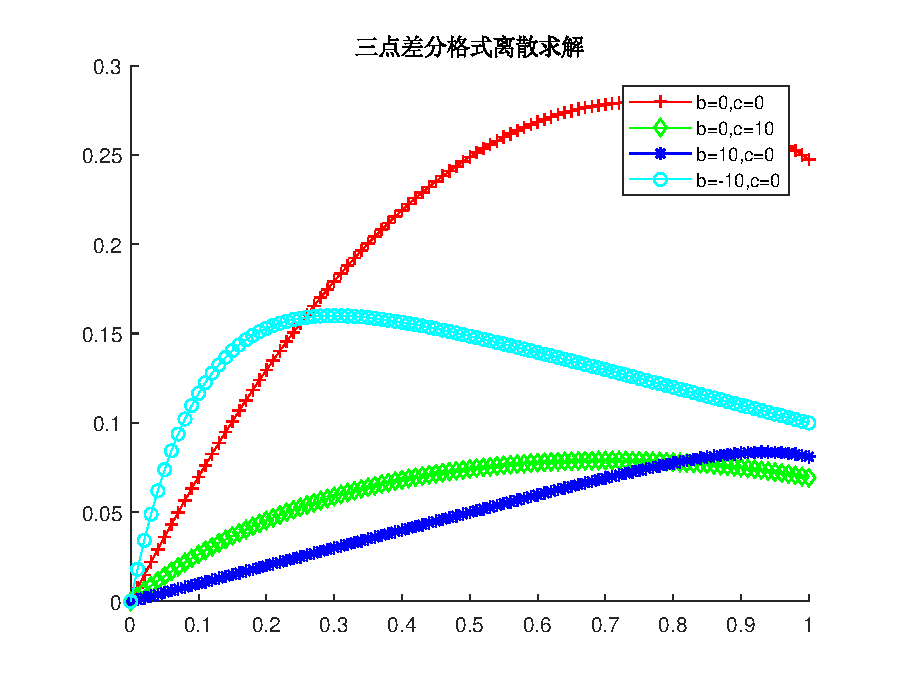
\includegraphics[width=1\linewidth]{week9_1_1.eps}
	\caption{三点差分格式离散求解}
	\label{Fig:1.1}
\end{figure}

差分格式精度分析,精确解如图\ref{Fig:1.2}。

\begin{figure}[H]
	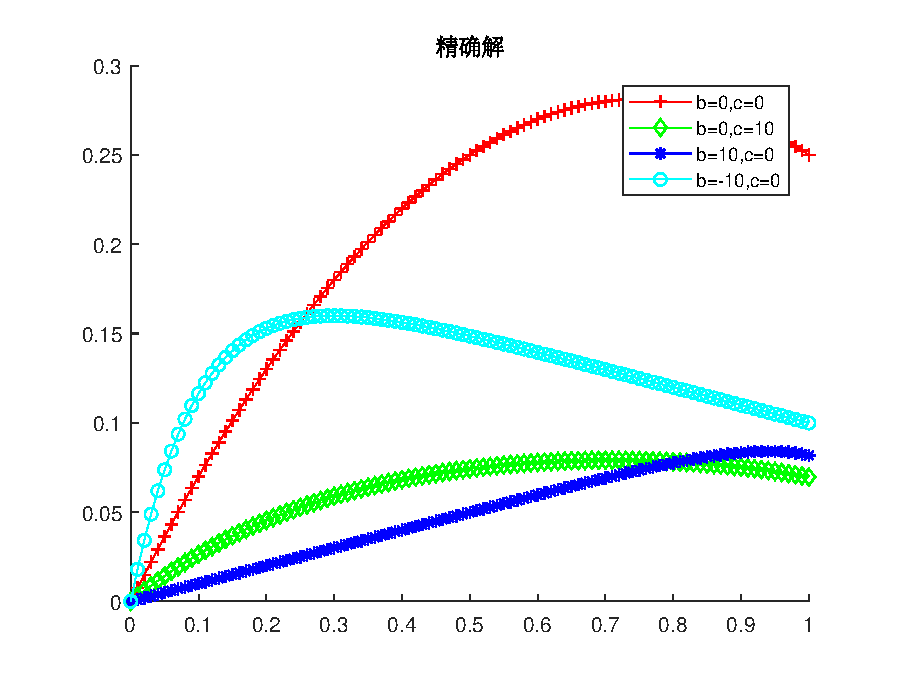
\includegraphics[width=1\linewidth]{week9_1_2.eps}
	\caption{精确解}
	\label{Fig:1.2}
\end{figure}

其中,

\noindent b=0,c=0时误差率是6.024096e-03\\
	b=0,c=10时误差率是1.755775e-03\\
	b=10,c=0时误差率是1.745959e-03\\
	b=-10,c=0时误差率是1.211599e-04\\


\end{proof}

\newpage

\section{P146 图3.5 标准三点差分格式和四阶HOC格式}

如图\ref{Fig:2.1}。

\begin{figure}[H]
	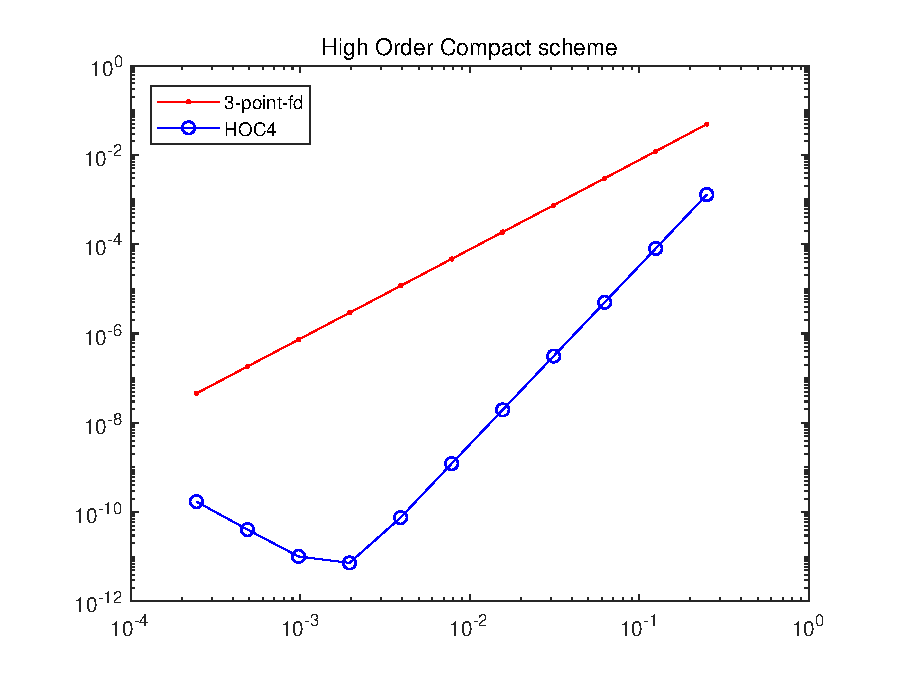
\includegraphics[width=1\linewidth]{week9_2_1.eps}
	\caption{标准三点差分格式和四阶HOC格式}
	\label{Fig:2.1}
\end{figure}


\end{document}
